% DRAFT generated as a starting point. Rewrite in my own voice before anyone reads it (see SPEC.md Section 9).
% Passive voice, undergraduate style, as requested.
% Compile from the notes/ folder: pdflatex research_note.tex
\documentclass[11pt,a4paper]{article}

\usepackage[margin=1in]{geometry}
\usepackage{graphicx}
\usepackage{booktabs}
\usepackage{tabularx}
\usepackage[hidelinks]{hyperref}
\usepackage{caption}
\usepackage{float}

\graphicspath{{../results/figures/}}
\newcommand{\degC}{\ensuremath{^{\circ}}C}
\captionsetup{font=small, labelfont=bf}

\title{Predicting the LCST of NIPAM copolymers from comonomer structure}
\author{}
\date{}

\begin{document}
\maketitle

\section{Introduction}

The temperature-responsive nanofibers developed in the Ebara group at NIMS are made
from NIPAM copolymerised with N-hydroxymethylacrylamide (HMAAm). Two roles are played
by the HMAAm. Its hydroxyl groups are used to crosslink the fibers when they are
heated, and because it is more hydrophilic than NIPAM, the LCST is raised from about
32\,\degC{} to the temperature required by the application. For magnetic
hyperthermia, this is around 42 to 45\,\degC. The choice of comonomer and of its
amount is therefore the central design decision.

In this project, the following question was investigated: given the structure of a
comonomer and its mole fraction in the chain, how well can the LCST be predicted, and
does the prediction still hold for a comonomer that was not seen during training?

\section{Data}

A single table of published LCSTs for random NIPAM copolymers in water or buffer was
built (\texttt{data/raw/lcst.csv}). The final table contains 113 training rows from 22
papers. These cover 22 comonomers, ranging from strongly hydrophilic (acrylamide,
HMAAm, hydroxyethylacrylamide) to strongly hydrophobic (butyl methacrylate, styrene,
aromatic amino-acid acrylamides). The measured LCSTs range from 15 to 80\,\degC{}
(Figures~\ref{fig:structures} and \ref{fig:overview}).

\begin{figure}[H]
  \centering
  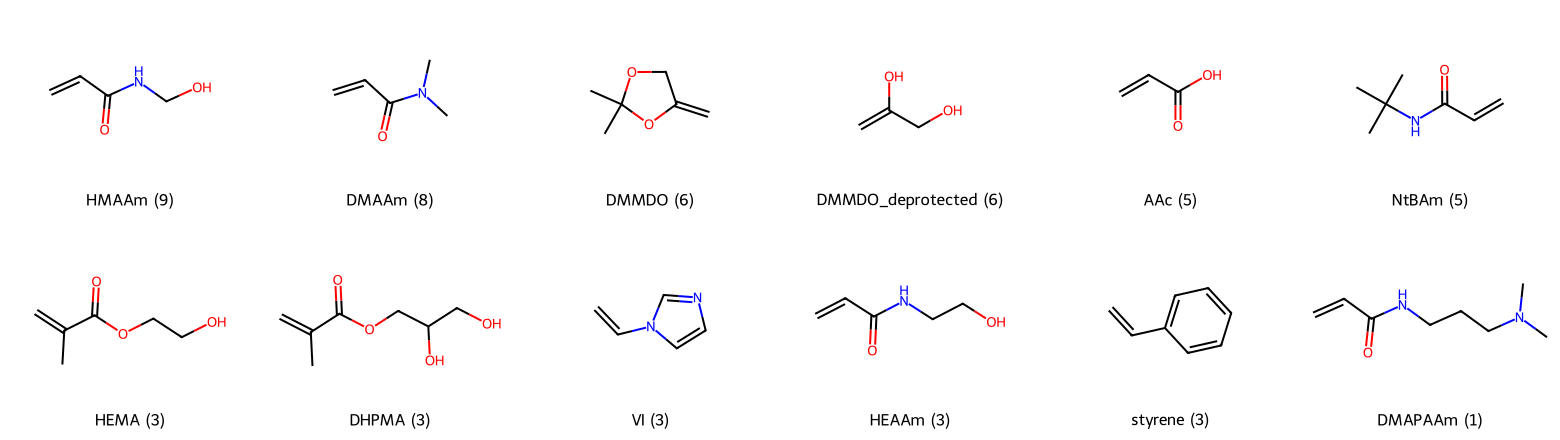
\includegraphics[width=\textwidth]{comonomer_structures.png}
  \caption{The 22 comonomers in the dataset, drawn as monomers. The number of rows
  for each comonomer is given in brackets.}
  \label{fig:structures}
\end{figure}

\begin{figure}[H]
  \centering
  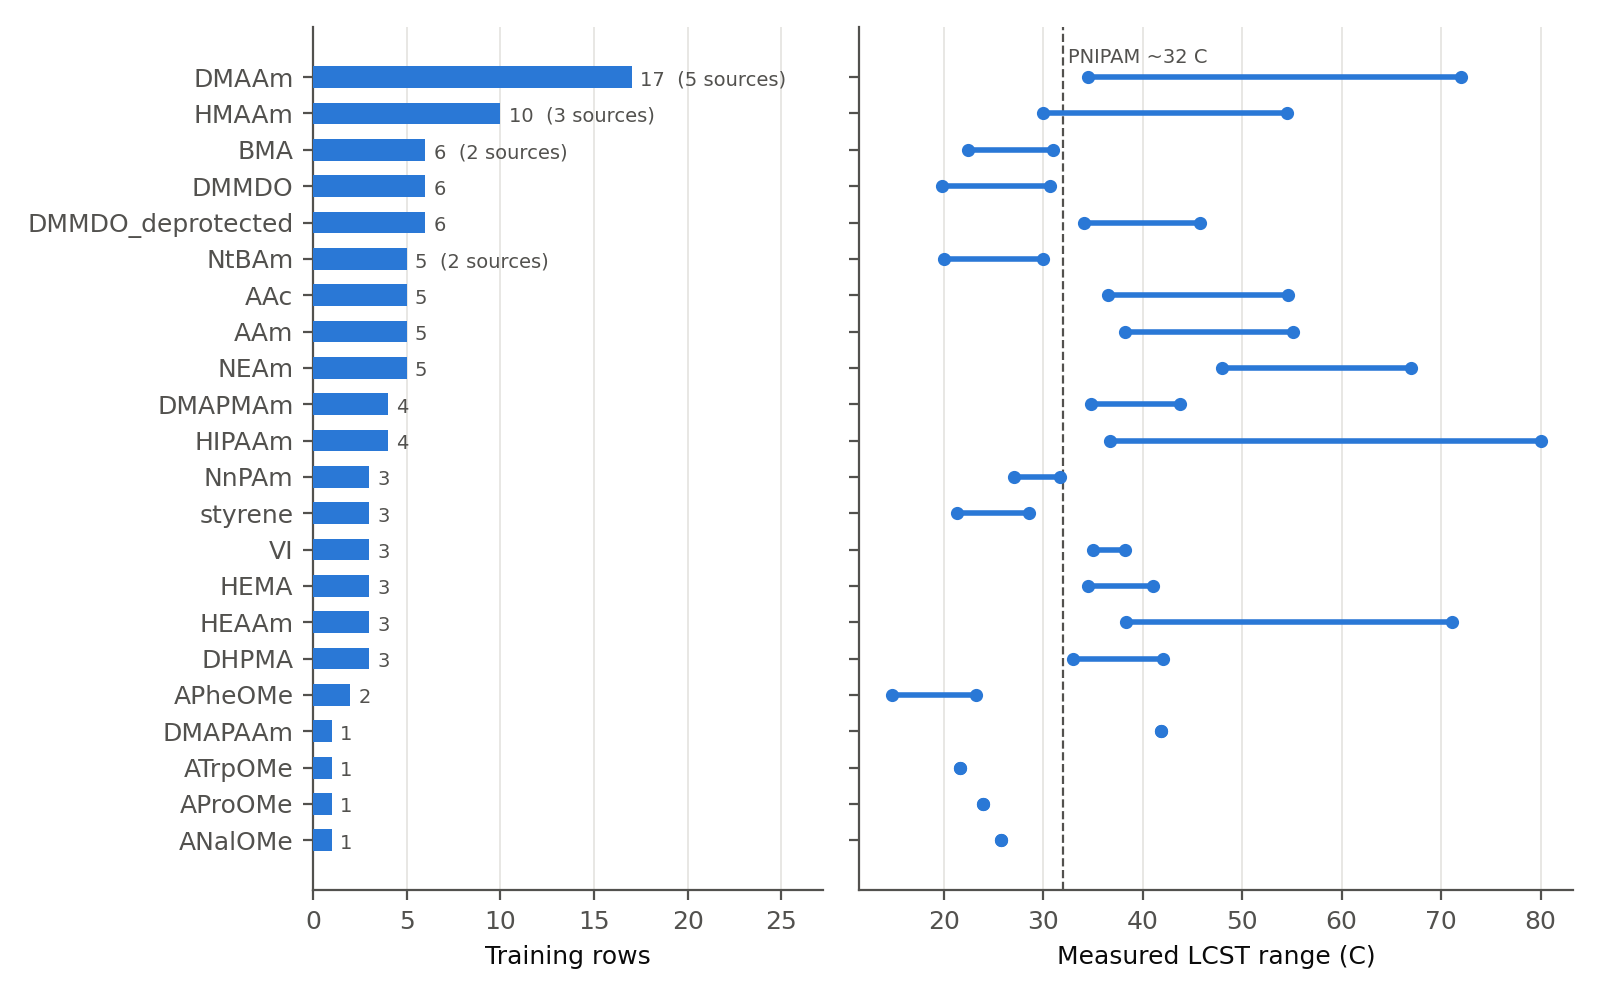
\includegraphics[width=0.85\textwidth]{dataset_overview.png}
  \caption{Training rows per comonomer (left) and the range of measured LCSTs for
  each comonomer (right). The dashed line marks PNIPAM at about 32\,\degC.}
  \label{fig:overview}
\end{figure}

Several problems with the data were kept in mind throughout.

\begin{enumerate}
  \item LCST was measured in at least five different ways. In some papers, the
  temperature at 50\% transmittance was reported, while in others the first sign of
  turbidity, an absorbance threshold, or a DSC peak was used. These values can differ
  by a few degrees for the same polymer. The method was recorded for every row, but
  no correction was applied.
  \item In some papers the monomer feed was reported, and in others the measured
  composition was reported. For free-radical copolymers these are usually close, but
  not always.
  \item 18 of the 22 comonomers were taken from a single paper each, and 19 rows are
  values that were compiled from the literature by another group without the
  measurement method being stated.
  \item The LCST of charged comonomers depends on pH. For this reason, acrylic acid
  and the two amine comonomers were left out of the headline analysis.
\end{enumerate}

After these were removed, the main set contained 103 rows and 19 comonomers. The
HMAAm copolymers reported by the Ebara group (seven values from four papers) were
placed in a separate check set and were not used for training.

\section{Method}

RDKit descriptors were calculated for each comonomer, and alvaDesc was also used,
which gives 4215 descriptors. The feature that was expected to matter most was a
simple one: the mole fraction multiplied by the difference between the logP of the
comonomer and that of NIPAM. The addition of 10\% of a comonomer that is much more
hydrophobic than NIPAM is expected to lower the LCST, and the addition of a more
hydrophilic comonomer is expected to raise it. The same construction was applied to
polar surface area (TPSA) and to the number of H-bond donors.

Every model was required to beat two baselines: a prediction of 32\,\degC{} for every
copolymer, and a straight line in mole fraction that ignores which comonomer is
present.

Particular attention was paid to validation. If one comonomer appears at five
compositions and the data are split randomly, that comonomer is seen by the model
during training, and only interpolation is required. This does not answer the
question that was asked. For this reason, random 5-fold cross-validation was reported
alongside grouped 5-fold cross-validation, in which all rows of a comonomer are held
out together, and alongside leave-one-comonomer-out validation. The grouped result was
taken as the main result.

\section{Results}

\subsection{Random versus grouped validation}

\begin{table}[H]
  \centering
  \small
  \caption{Mean absolute error (\degC) for the uncharged comonomers (103 rows, 19 comonomers).}
  \label{tab:metrics}
  \begin{tabular}{@{}lcc@{}}
    \toprule
    Model & Random 5-fold & Grouped 5-fold \\
    \midrule
    32\,\degC{} for everything & 8.9 & 8.9 \\
    Linear in mole fraction & 6.2 & 6.6 \\
    Ridge, fraction $\times$ (logP, TPSA, HBD difference) & 3.6 & \textbf{4.3} \\
    Random forest, 8 RDKit descriptors & 4.0 & 5.0 \\
    Ridge, all 8 RDKit descriptors & 3.8 & 6.8 \\
    Ridge, top 10 alvaDesc descriptors (selected inside each fold) & 4.5 & 20.8 \\
    \bottomrule
  \end{tabular}
\end{table}

Under random splits, almost every model appeared accurate, with errors between 3.6
and 4.5\,\degC{} (Table~\ref{tab:metrics}, Figure~\ref{fig:summary}). Under grouped
splits, the models were clearly separated. The error of the small ridge model on four
fraction-weighted features increased by only 0.7\,\degC. In contrast, the error of
the alvaDesc ridge model increased from 4.5 to 20.8\,\degC. It was found that this
model had learned the comonomers it was trained on and gave extreme predictions for
new ones, mostly for comonomers at high fraction whose descriptor values were outside
the training range. It had been expected that the large descriptor set would improve
the predictions, but this was not the case.

With the fraction multiplied by logP alone, the mole-fraction baseline was beaten by
only about half a degree. When polar surface area and H-bond donors were added, the
error was reduced from 6.0 to 4.3\,\degC{} (Figure~\ref{fig:parity}).

\begin{figure}[H]
  \centering
  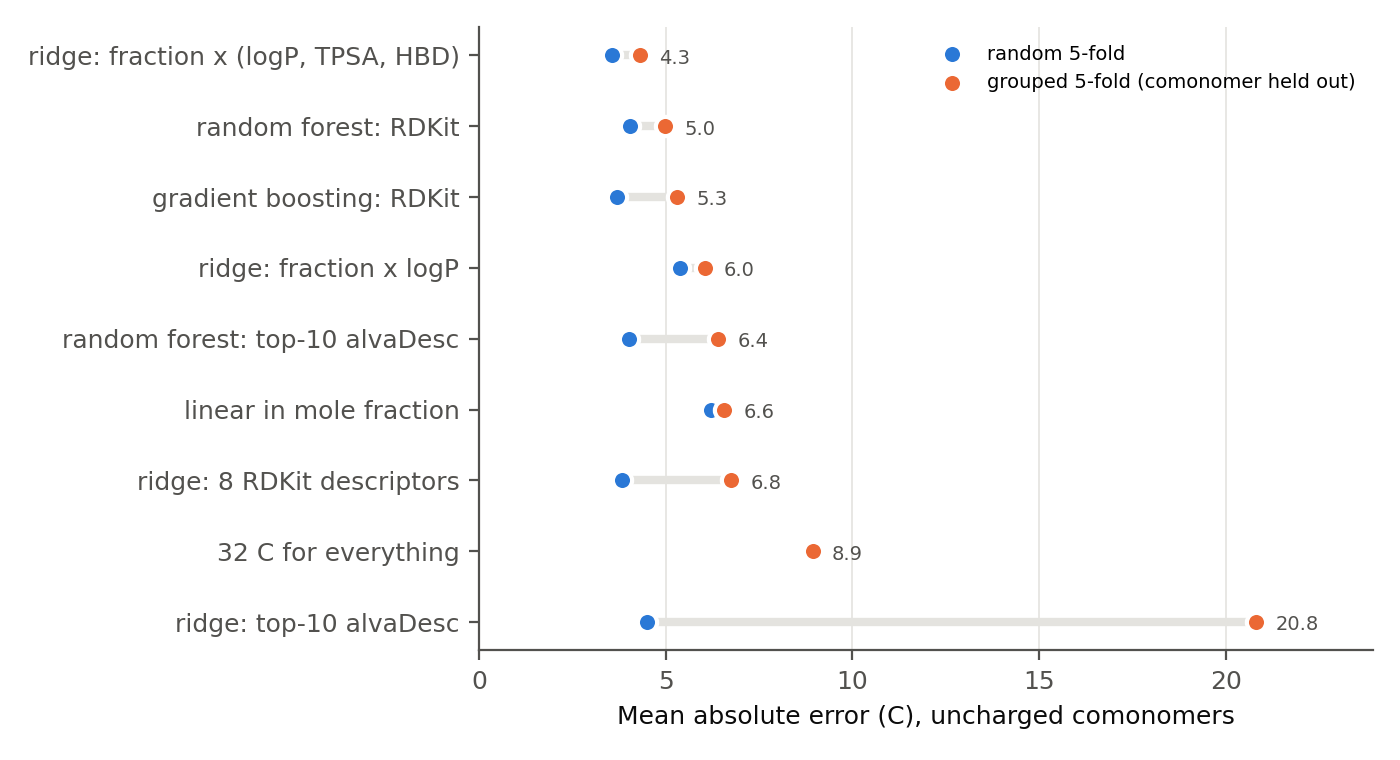
\includegraphics[width=0.8\textwidth]{results_summary.png}
  \caption{Random (blue) and grouped (orange) 5-fold errors for every model. The
  length of each grey bar shows how much of the random-split accuracy was due to the
  model having already seen the comonomer.}
  \label{fig:summary}
\end{figure}

\begin{figure}[H]
  \centering
  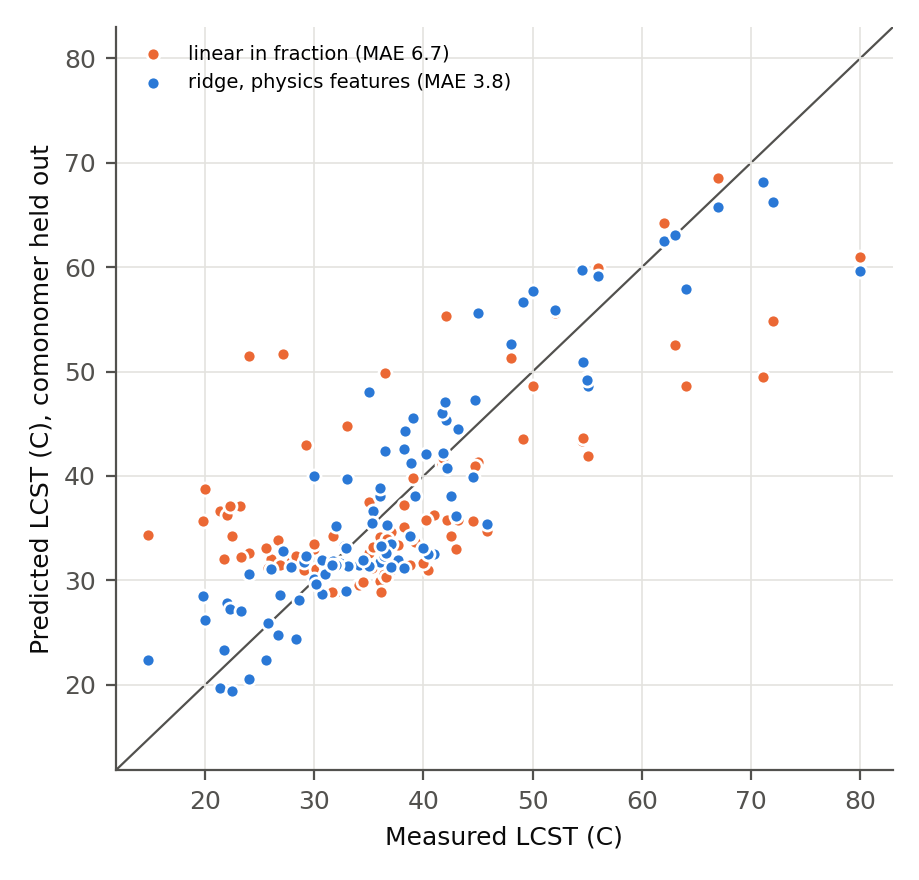
\includegraphics[width=0.5\textwidth]{parity_logo.png}
  \caption{Leave-one-comonomer-out predictions against measured LCST for the physics
  ridge model (blue) and the mole-fraction baseline (orange).}
  \label{fig:parity}
\end{figure}

\subsection{Reproduction of the known trends}

It is reported in the literature that hydrophobic comonomers lower the LCST and
hydrophilic comonomers raise it. This was confirmed in the collected data: for each
comonomer, the LCST shift per 10\,mol\% was fitted, and it was found to decrease with
logP (Spearman $\rho = -0.82$ over 19 comonomers). When each comonomer was predicted
at 10\,mol\% with that comonomer held out, the same order was obtained from the model
($\rho = -0.92$, Figure~\ref{fig:trend1}).

\begin{figure}[H]
  \centering
  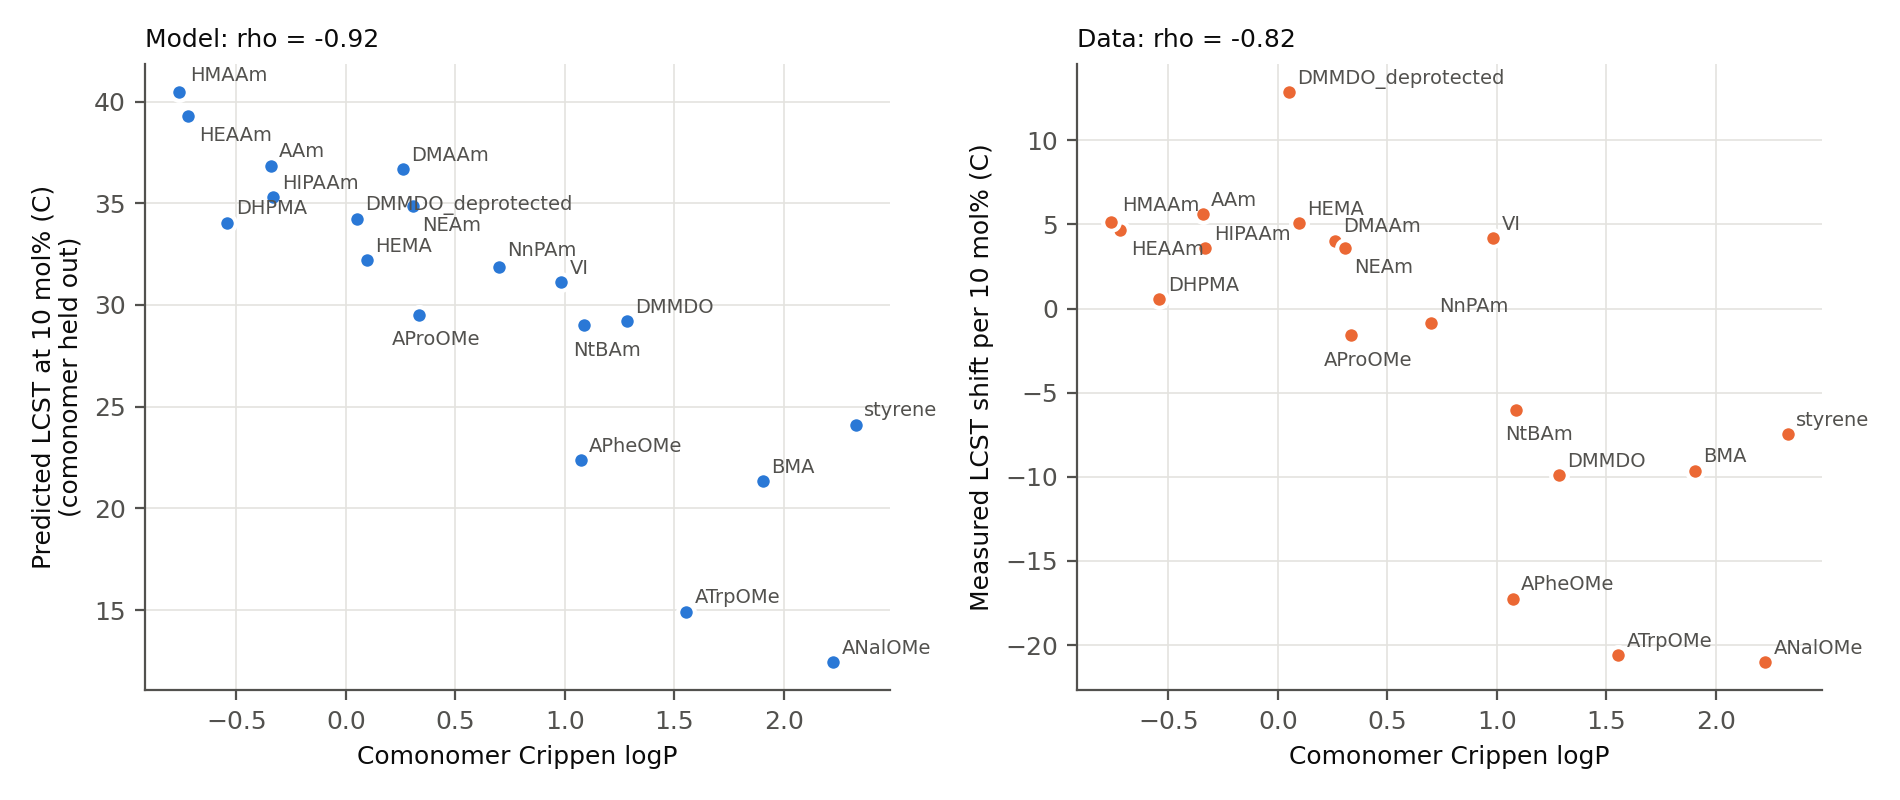
\includegraphics[width=\textwidth]{trend1_logp.png}
  \caption{Left: predicted LCST at 10\,mol\% for each comonomer, with that comonomer
  held out. Right: measured LCST shift per 10\,mol\%. Both are plotted against the
  Crippen logP of the comonomer.}
  \label{fig:trend1}
\end{figure}

For the composition dependence, the held-out predictions were compared with the
measured series (Figure~\ref{fig:trend2}). For DMAAm (17 rows from 5 papers), a shift
of 5.1\,\degC{} per 10\,mol\% was predicted, which is the same as the measured value.
For N-ethylacrylamide, 3.6\,\degC{} was predicted against 3.4\,\degC{} measured. The
direction was correct for all six series that were examined, but the size of the
shift was underestimated for N-tert-butylacrylamide and HIPAAm and overestimated for
HMAAm (8.1 against 5.1\,\degC{} per 10\,mol\%).

\begin{figure}[H]
  \centering
  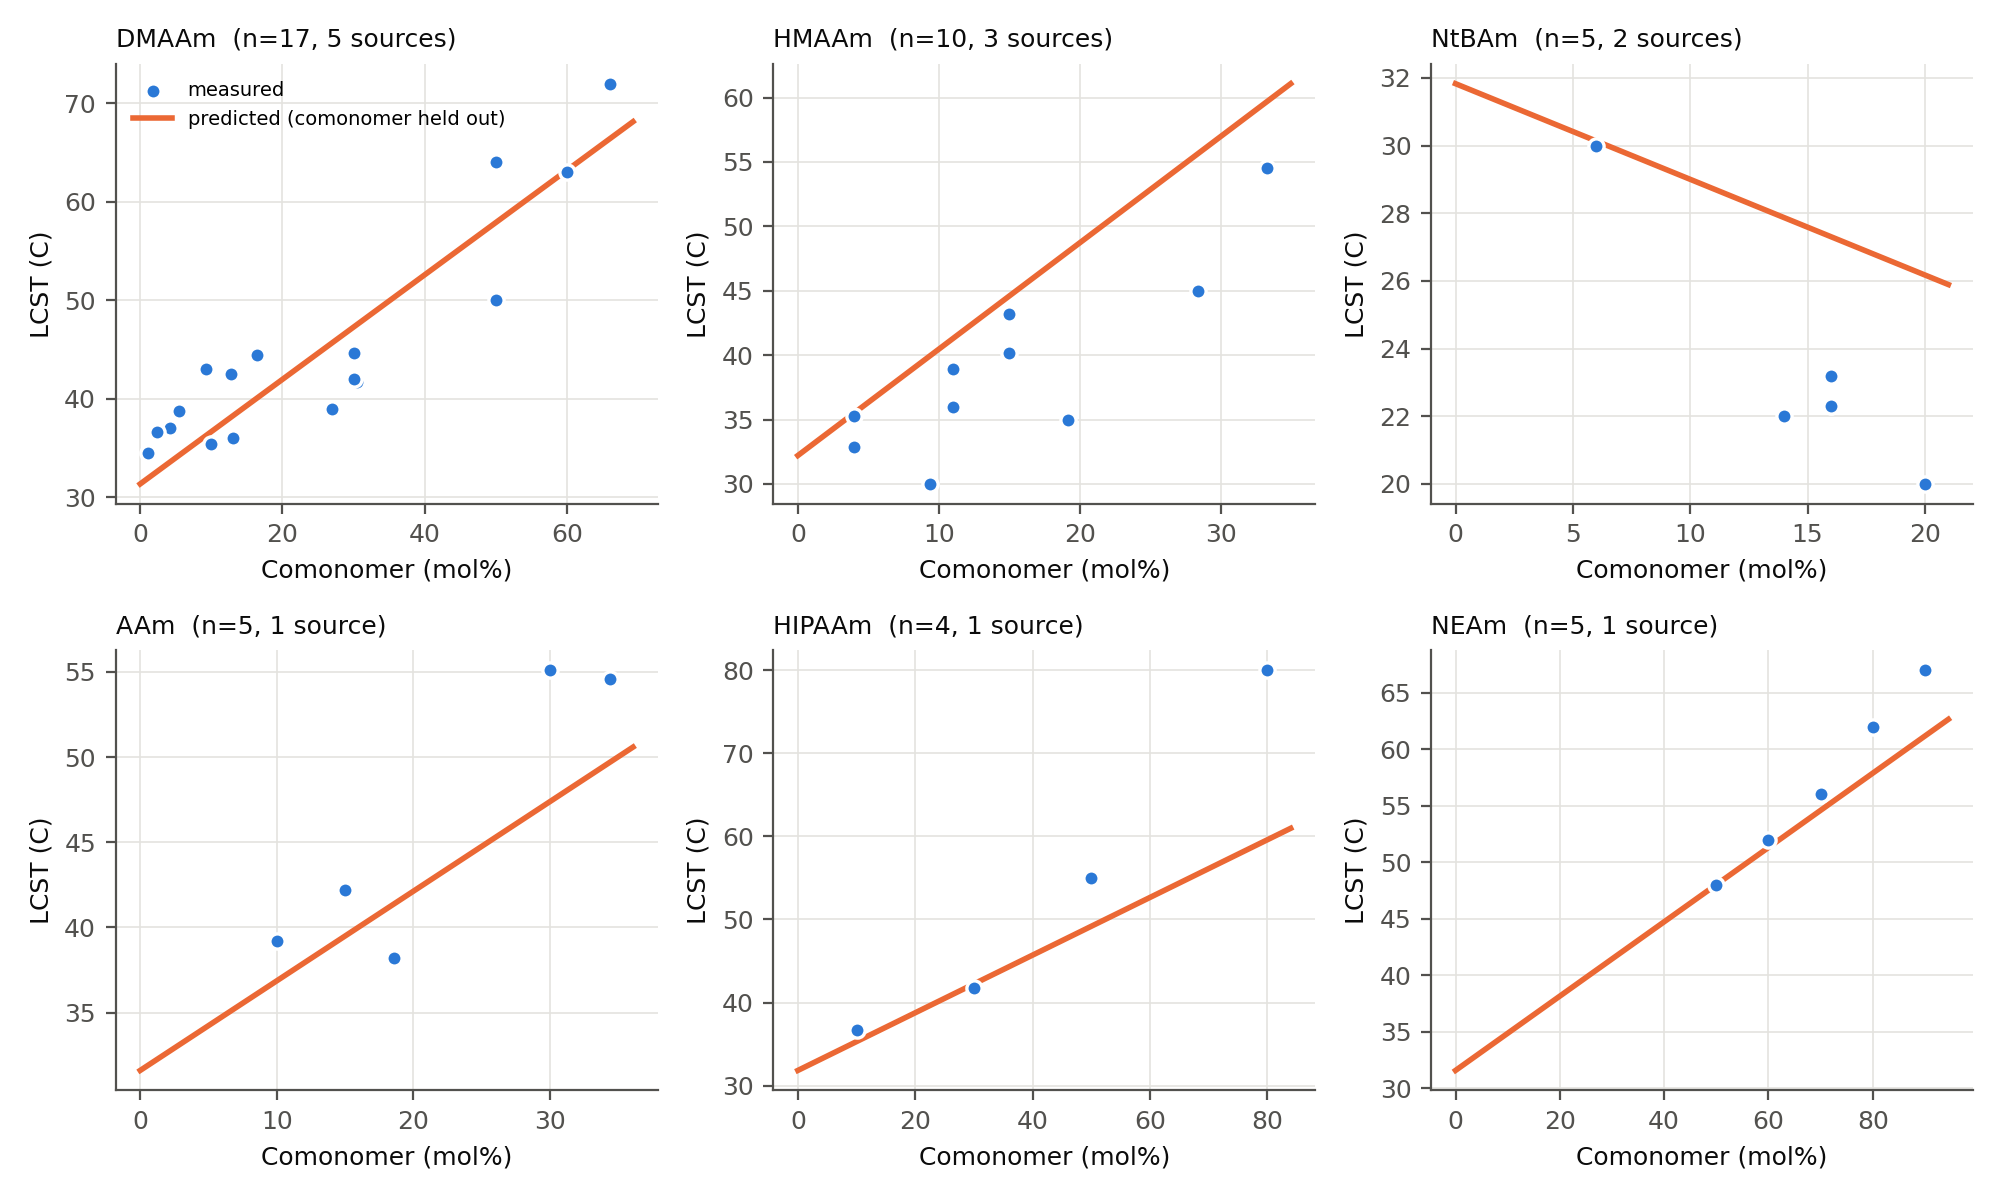
\includegraphics[width=\textwidth]{trend2_series.png}
  \caption{Measured composition series (points) and predictions from a model trained
  without that comonomer (line).}
  \label{fig:trend2}
\end{figure}

One result was found that does not fit the textbook picture. A negative coefficient
was obtained for polar surface area (Figure~\ref{fig:coef}), which, if read on its
own, would mean that a larger polar surface lowers the LCST. This result was stable
(the same sign was obtained in 99\% of bootstrap refits in which the comonomers were
resampled) and was not caused by the bulky aromatic comonomers. It is thought that
this term acts as a correction to the logP term, since the two fraction-weighted
features are correlated with $r = -0.74$, and a single hydrophilicity effect is
therefore divided between them. When TPSA was removed, the grouped error increased
from 4.3 to 7.2\,\degC, so the term is useful for prediction, but the coefficients
should not be interpreted one by one.

\begin{figure}[H]
  \centering
  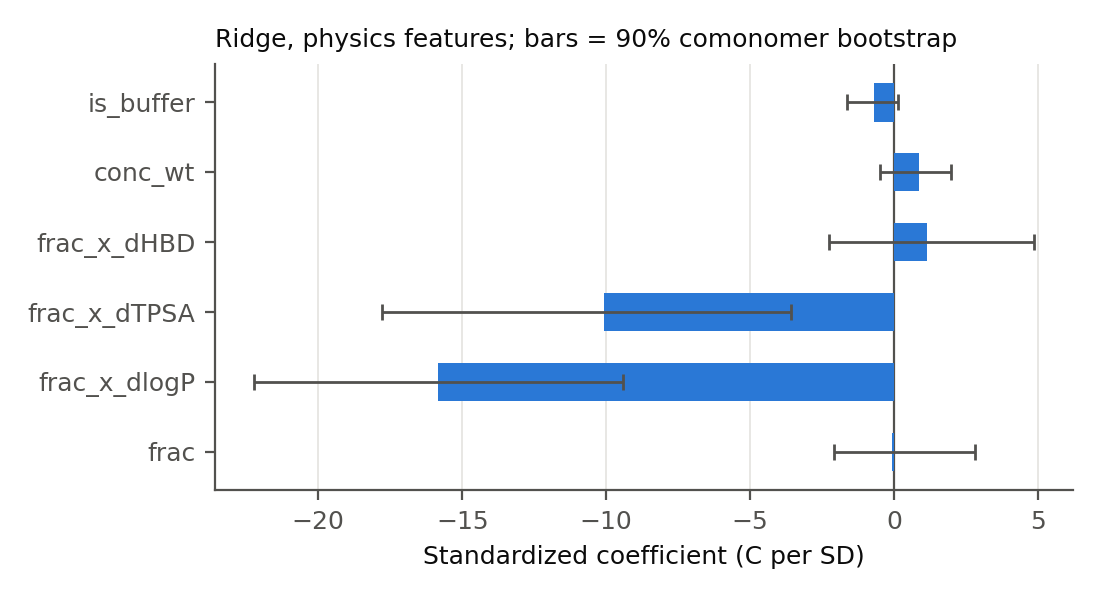
\includegraphics[width=0.62\textwidth]{coefficients_ridge_physics.png}
  \caption{Standardised coefficients of the physics ridge model, with 90\% intervals
  from 200 bootstrap refits in which comonomers were resampled.}
  \label{fig:coef}
\end{figure}

\subsection{The Ebara check}

All HMAAm rows were removed from training, so that HMAAm had not been seen by the
model, and the seven values reported by the Ebara group were then predicted
(Table~\ref{tab:ebara}, Figure~\ref{fig:ebara}).

\begin{table}[H]
  \centering
  \small
  \caption{Ebara group HMAAm copolymers: measured LCST and prediction of a model
  trained without any HMAAm data (\degC). The Kim 2012 values are the end points of
  the stated range of 34 to 38\,\degC{} for 3 to 10\,mol\%.}
  \label{tab:ebara}
  \begin{tabular}{@{}lcccc@{}}
    \toprule
    Source & HMAAm (mol\%) & Solvent & Measured & Predicted (90\% interval) \\
    \midrule
    Techawanitchai 2011 & 10 & water & 36.1 & 40.4 (32.1--49.1) \\
    Techawanitchai 2011 & 20 & water & 45.5 & 48.6 (40.4--58.6) \\
    Techawanitchai 2011 & 30 & water & 56.0 & 56.9 (49.0--69.7) \\
    Niiyama 2018 & 21 & PBS & 43.0 & 47.1 (37.0--57.5) \\
    Chen 2022 & 20 & PBS & 42.1 & 46.2 (36.0--56.6) \\
    Kim 2012 & 3 & PBS & 34.0 & 32.2 (20.6--40.9) \\
    Kim 2012 & 10 & PBS & 38.0 & 38.0 (26.8--47.1) \\
    \bottomrule
  \end{tabular}
\end{table}

A mean error of 2.6\,\degC{} was obtained, compared with 5.8\,\degC{} for the
mole-fraction baseline and 10.1\,\degC{} for a prediction of 32\,\degC. All seven
measured values were found inside the 90\% prediction interval. The copolymer with
30\,mol\% HMAAm in water, which was measured at 56.0\,\degC, was predicted at
56.9\,\degC. Near 20\,mol\% HMAAm, the predictions were 3 to 4\,\degC{} too high,
mostly for the measurements made in PBS.

\begin{figure}[H]
  \centering
  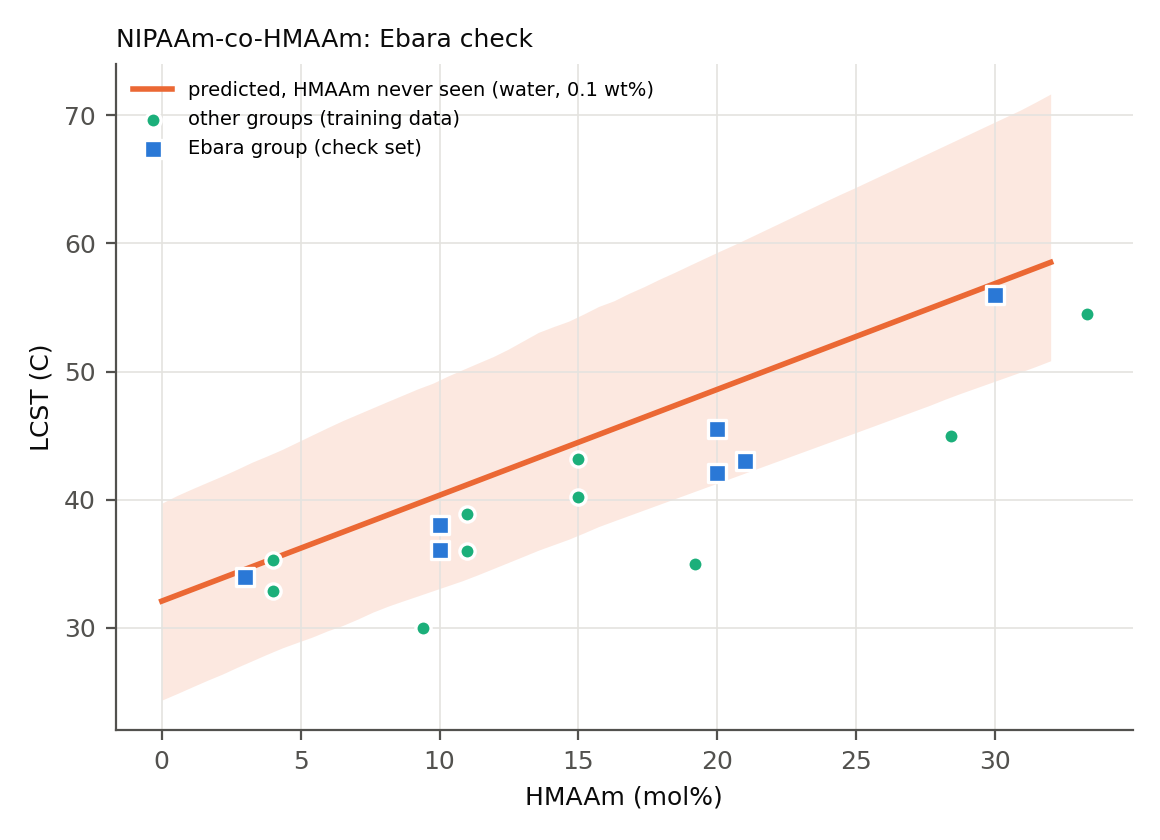
\includegraphics[width=0.62\textwidth]{ebara_check.png}
  \caption{Ebara group data (squares), HMAAm data from other groups (circles, not
  used for this prediction), and the prediction of the model trained without HMAAm
  (line, 90\% interval shaded).}
  \label{fig:ebara}
\end{figure}

This difference is partly a result of the spread in the published HMAAm data rather
than of the model. Across the papers that were used, the LCST increase per 10\,mol\%
HMAAm ranges from about 3 to 7\,\degC, which is expected given the differences in
measurement method, concentration, and molecular weight. When the HMAAm data from the
other groups were added back into training, the error was reduced only from 2.6 to
2.1\,\degC.

\subsection{A new prediction}

The model was then used to find a comonomer, not included in the data, that would
place the transition at 38 to 40\,\degC, just above body temperature. It is predicted
that this is achieved with N-acryloylmorpholine (NAM) at 14 to 17\,mol\% (in water,
0.1\,wt\%). At 20\,mol\%, an LCST of 41\,\degC{} is predicted, with a 90\% interval of
31 to 50\,\degC{} (Figure~\ref{fig:nam}).

\begin{figure}[H]
  \centering
  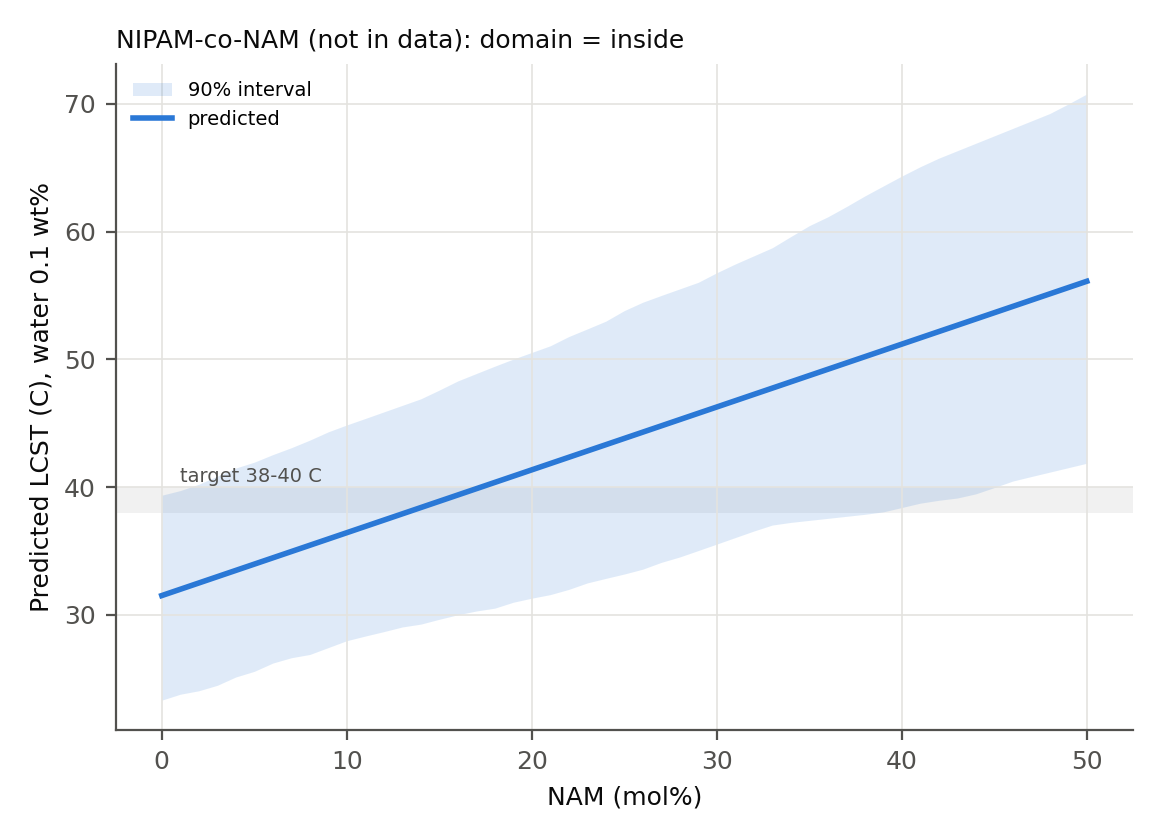
\includegraphics[width=0.62\textwidth]{new_prediction.png}
  \caption{Predicted LCST of NIPAM-co-NAM against NAM content, with the 90\% interval.
  The grey band marks the 38 to 40\,\degC{} target.}
  \label{fig:nam}
\end{figure}

The logP, polar surface area, and H-bond donor count of NAM all lie within the range
of the training comonomers, and its leverage is 0.29 compared with a threshold of
0.63. Therefore, NAM is considered to be inside the applicability domain of the model
in terms of its descriptors. However, it is structurally new, since the fingerprint
similarity to the nearest training comonomer is only 0.31. The prediction should
therefore be regarded as lying within the descriptor range but for a chemistry that is
not covered by the data.

N-(2-hydroxypropyl)methacrylamide (HPMA) was considered first, because it is
hydrophilic and carries a hydroxyl group like HMAAm. However, almost no change in LCST
was predicted for HPMA. When the individual terms were examined, it was found that its
logP contribution (+10.7\,\degC{} at 20\,mol\%) is cancelled by its TPSA contribution
($-9.7$\,\degC), which is the correlated term discussed above. For NAM, the prediction
comes almost entirely from the logP term, so NAM was chosen instead.

\section{Limitations}

\begin{itemize}
  \item 22 comonomers is a small set, and the headline error of 4.3\,\degC{} is based
  on 19 of them.
  \item A few degrees of noise are added by the mixed measurement methods, and this
  cannot be explained by any descriptor.
  \item Molecular weight and end groups are known to affect the LCST, especially for
  short chains, but molecular weight was missing for about half of the rows and could
  not be used.
  \item Isomers cannot be separated by two-dimensional descriptors. The same logP is
  given to N-n-propylacrylamide and NIPAM, even though the homopolymer of
  N-n-propylacrylamide switches about 10\,\degC{} lower.
  \item The model is linear in mole fraction. This is adequate up to about 30\,mol\%
  for most comonomers, but curvature is seen in the measured data at higher fractions.
\end{itemize}

\section{Future work}

The most direct test would be the synthesis of NIPAM-co-NAM at around 15\,mol\%,
followed by measurement of its cloud point by UV-vis spectroscopy with a temperature
ramp, to determine whether the transition lies at 38 to 40\,\degC. It would also be of
interest to study how the HMAAm content and crosslinking affect the transition once
the polymer is electrospun into fibers, since the solution LCST is only the first
step for the systems developed in the Ebara group.

\end{document}
